\documentclass[11pt,a4paper]{article}
\usepackage{amsmath,amsthm,amsfonts,amssymb,amscd}
\usepackage{enumerate} 
\usepackage{physics}
\usepackage{enumerate}
\usepackage{fancyhdr}
\usepackage{hyperref}
\usepackage{graphicx}
\usepackage{xurl}
\hypersetup{colorlinks,
    linkcolor=blue,
    citecolor=blue,      
    urlcolor=blue,
}

\oddsidemargin0.1cm 
\evensidemargin0.8cm
\textheight22.7cm 
\textwidth15cm \topmargin-0.5cm

\newtheorem{theorem}{Theorem}
\newtheorem{corollary}{Corollary}
\newtheorem{lemma}{Lemma}
\newtheorem{proposition}{Proposition}

\theoremstyle{definition}
\newtheorem{remark}{Remark}
\newtheorem{definition}{Definition}
\newtheorem{observation}{Observation}
\newtheorem{note}{Note}
\newtheorem{hope}{Hope}
\newtheorem{warning}{Warning}
\newtheorem{problem}{Problem}
\newtheorem{fear}{Fear}
\newtheorem{question}{Question}

\newcommand{\Z}{\mathbb{Z}}
\newcommand{\R}{\mathbb{R}}
\newcommand{\C}{\mathbb{C}}
\newcommand{\Q}{\mathbb{Q}}
\newcommand{\A}{\mathbb{A}}

\usepackage{listings}
\usepackage{xcolor}

\definecolor{codegreen}{rgb}{0,0.6,0}
\definecolor{codegray}{rgb}{0.5,0.5,0.5}
\definecolor{codepurple}{rgb}{0.58,0,0.82}
\definecolor{backcolour}{rgb}{0.95,0.95,0.92}

\lstdefinestyle{mystyle}{
    backgroundcolor=\color{backcolour},   
    commentstyle=\color{codegreen},
    keywordstyle=\color{magenta},
    numberstyle=\tiny\color{codegray},
    stringstyle=\color{codepurple},
    basicstyle=\ttfamily\footnotesize,
    breakatwhitespace=false,         
    breaklines=true,                 
    captionpos=b,                    
    keepspaces=true,                 
    numbers=left,                    
    numbersep=5pt,                  
    showspaces=false,                
    showstringspaces=false,
    showtabs=false,                  
    tabsize=2
}

\lstset{style=mystyle}

\newcommand{\MultiSet}{\mathrm{MultiSet}}
\newcommand{\len}{\mathrm{len}}
\newcommand{\din}{\texttt{d\_in}}
\newcommand{\dout}{\texttt{d\_out}}
\newcommand{\Relation}{\mathrm{Relation}}
\newcommand{\X}{\mathcal{X}}
\newcommand{\Y}{\mathcal{Y}}
\newcommand{\U}{\texttt{U}}
\newcommand{\True}{\texttt{True}}
\newcommand{\False}{\texttt{False}}
\newcommand{\clamp}{\texttt{clamp}}
\newcommand{\function}{\texttt{function}}
\newcommand{\float}{\texttt{float }}
\newcommand{\questionc}[1]{\textcolor{red}{\textbf{Question:} #1}}

\newcommand{\silvia}[1]{{ {\color{blue}{(silvia)~#1}}}}
\newcommand{\grace}[1]{{ {\color{purple}{(grace)~#1}}}}
\newcommand{\connor}[1]{{ {\color{teal}{(connor)~#1}}}}

\newcommand{\todo}{{\textcolor{red}{TODO }}}


\title{Privacy Proofs for OpenDP: Bounded Sum with Known $n$}
\author{S\'ilvia Casacuberta}
\date{Summer 2021}

\begin{document}

\maketitle

\tableofcontents

\section{Algorithm Implementation}
\subsection{Code in Rust}
The current OpenDP library contains the transformation \texttt{make\_bounded\_sum\_n} implementing the bounded sum function with known $n$. This is defined in lines 53-68 of the file \texttt{sum.rs} in the Git repository\footnote{As of July 1, 2021.} (\url{https://github.com/opendp/opendp/blob/b936c74223b4e319698fa51837b5f8f40f3126d3/rust/opendp/src/trans/sum.rs#L53-L68}).

\begin{figure}[ht]
    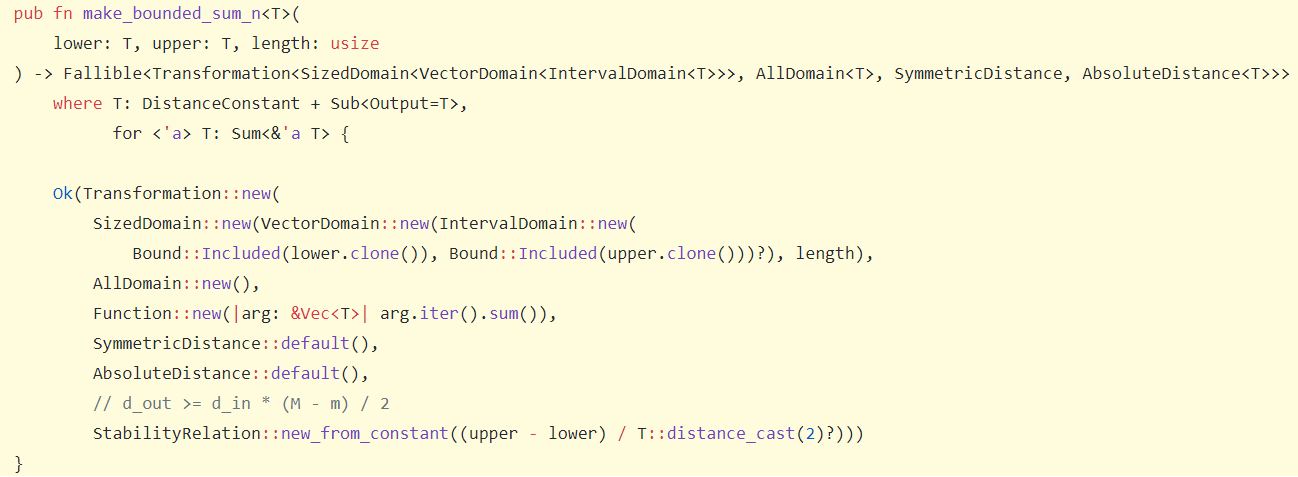
\includegraphics[width=15cm]{sumn.png}
    \centering
    \label{fig:code}
\end{figure}

% what do to with n? Take it as input to T(x)?
% Is it correct to say x_i? I mean the i-th element in the multiset

\subsection{Pseudocode in Python}
We present a simplified Python-like pseudocode of the Rust implementation below. The necessary definitions for the pseudocode can be found at \href{https://www.overleaf.com/project/60d215bf90b337ac02200a99}{``List of definitions used in the pseudocode"}.

\subsubsection*{Preconditions}
To ensure the correctness of the output, we require the following preconditions:

\begin{itemize}
    \item \textbf{User-specified types:}
    \begin{itemize}
        \item Variable \texttt{n} must be of type \texttt{usize}.
        \item Type \texttt{T} must have traits \texttt{TotalOrd} and \texttt{Sub(Output=T)}.\footnote{For now, the OpenDP library only implements \texttt{PartialOrd}, but \texttt{TotalOrd} will soon be implemented.}
\end{itemize}
\end{itemize}

\subsubsection*{Postconditions}
\begin{itemize}
    \item A \texttt{Transformation} is returned (i.e., if a \texttt{Transformation} cannot be returned successfully, then an error should be returned).
\end{itemize}

\begin{lstlisting}[language=Python, escapechar=|]
def MakeBoundedSumN(L: T, U: T, n: usize):
    input_domain = SizedDomain(VectorDomain(IntervalDomain(L, U)), n)
    output_domain = AllDomain(T)
    input_metric = SymmetricDistance()
    output_metric = AbsoluteDistance(T)
    
    if L*n < get_min_value(T) or U*n > get_max_value(T): 
        raise Exception('Invalid parameters') |\label{line:max}|
    
    def Relation(d_in: u32, d_out: u32) -> bool: |\label{line:rel}|
        return d_out >= d_in*(U-L)/2
    
    def function(data: Vec(T)) -> T: |\label{line:fn}|
        return data.iter().sum() |\label{line:sum}|
    return Transformation(input_domain, output_domain, function, input_metric, output_metric, stability_relation)
\end{lstlisting}

\iffalse
\subsubsection*{Conditions as specified in the pseudocode}
\begin{itemize}
    \item \underline{Input domain:} sized domain of all vectors of elements in \texttt{IntervalDomain(L, U)}, where \texttt{L} and \texttt{U} are of type \texttt{T} and stand for \textit{lower bound} and \textit{upper bound}, respectively.\footnote{The compiler infers \texttt{float} from the context, which is why it is omitted.} 
    
    \item \underline{Output domain:} domain of all elements of type \texttt{T}.
    
    \item \underline{Function:} given $v$ of type \texttt{Vec(T)}, it returns an element of type \texttt{T} which corresponds to the sum of all the vector entries $v_i$ of $v$.
    
    \item \underline{Input metric:} symmetric distance.\footnote{As of June 24, SubstituteDistance is no longer a metric part of the OpenDP library.}
    
    \item \underline{Output metric:} absolute distance.
    
    \item \underline{Stability relation:} for $\din, \dout$ of type \texttt{u32}, the relation returns $\True$ if and only if $\dout \geq \din \cdot (\U-\texttt{L})/2$.
\end{itemize}
\fi

%More concisely, the stability relation can be stated as:%\footnote{See page 14 of \textit{A Programming Framework for OpenDP} for more examples. Note that in the Rust implementation the metrics $d_{\X}$ and $d_{\Y}$ are \textit{not} inputs to the relation, and they are instead fixed as attributes of the transformation.}
%\begin{equation}\label{eq:relation}
    %\textrm{R}(\din, \dout) = 
    %\begin{cases} 
      %\True & \textrm{if } \dout \geq \din \cdot (\U - \texttt{L})/2 \textrm{ for } \din, \dout \textrm{ of type } \texttt{u32} \\
      %\False & \textrm{otherwise}
   %\end{cases}
%\end{equation}
%\silvia{Maybe take out the equation form; repetitive.}

\section{Proof}
\subsection{Symmetric Distance}
\begin{theorem}
    For every setting of the input parameters \texttt{(L, U, n)} to \texttt{MakeBoundedSumN}, the transformation returned by \texttt{MakeBoundedSumN} has the following properties:
    \begin{enumerate}
        \item \textup{(Appropriate output domain).} For every element $v$ in \texttt{input\_domain}, $\function(v)$ is in \texttt{output\_domain}. % Prof. Vadhan said on 29/6 to leave it as this for now, but maybe in the future we add to the theorem statement what exactly the input domain and output domain are (although of course we already say this in the proof)
        \item \textup{(Domain-metric compatibility).} The domain \texttt{input\_domain} matches one of the possible domains listed in the definition of \texttt{input\_metric}, and likewise \texttt{output\_domain} matches one of the possible domains listed in the definition of \texttt{output\_metric}.
        
        \item \textup{(Stability guarantee).} For every pair of elements $v, w$ in \texttt{input\_domain} and for every pair $(\din, \dout)$, where $\din$ is of type \texttt{u32} and $\dout$ is of type \texttt{T}, if $v,w$ are $d_{in}$-close under \texttt{input\_metric} and $\Relation(\din, \dout) = \True$, then $\function(v)$, \texttt{function}$(v)$ are $d_{out}$-close under \texttt{output\_metric}.
    \end{enumerate}
\end{theorem}

\begin{proof}
    \textbf{(Appropriate output domain).} In the case of \texttt{MakeBoundedSumN}, this corresponds to showing that for every vector $v$ in \texttt{SizedDomain(VectorDomain(IntervalDomain (L, U)), n)}, where \texttt{L} and \texttt{U} have type \texttt{T}, then \texttt{function}$(v)$ belongs to \texttt{AllDomain(T)}. %Unpacking the domain definitions, this means that, by assumption, vector $v$ has: 1) length \texttt{length}, 2) entries of type \texttt{float}, and 3) entries that belong to the interval $[L, U]$. 
    The output correctness follows from the type signature of \texttt{function} as defined in line \ref{line:fn} and from the overflow check in line \ref{line:max}. The latter ensures that \texttt{function(v)} is contained in the interval \texttt{[get\_min\_value(T), get\_max\_value(T)]}, and hence no overflow occurs in line \ref{line:sum}. The former automatically enforces that \texttt{function(v)} has type \texttt{T}. Since the Rust code successfully compiles, by the type signature the appropriate output domain property must hold. Otherwise, the code will raise an exception for incorrect input type.
    
    \smallskip
    \textbf{(Domain-metric compatibility).} For \texttt{MakeBoundedSumN}, this corresponds to showing that \texttt{SizedDomain(VectorDomain(IntervalDomain (L, U)), n)} is compatible with symmetric distance, and that \texttt{AllDomain(T)} is compatible with absolute distance. Both follow directly from the definition of symmetric distance and absolute distance (note that, for symmetric distance, \texttt{SizedDomain(VectorDomain(D))} is a subset of \texttt{VectorDomain(D)}), as stated in \href{https://www.overleaf.com/project/60d214e390b337703d200982}{``List of definitions used in the proofs"}, along with the \textit{appropriate output domain property} shown above, which ensures that \texttt{output\_domain} is indeed \texttt{AllDomain(T)}.
    
    \smallskip
    \textbf{(Stability guarantee).} Throughout the stability guarantee proof, we can assume that $\function(v)$ and $\function(w)$ are in the correct output domain, by the \textit{appropriate output domain property} shown above. 
    
    Since by assumption $\Relation(\din, \dout) = \True$, by the \texttt{MakeBoundedSumN} stability relation (as defined in line~\ref{line:rel} in the pseudocode), we have that $\dout \geq \din \cdot (\U - \texttt{L})/2$. Moreover, $v, w$ are assumed to be $\din$-close. By the definition of the symmetric difference metric, this is equivalent to stating that $d_{Sym}(v, w) = |\MultiSet(v) \Delta \MultiSet(w)| \leq \din$.

    Further, applying the histogram notation,\footnote{See \textit{A Programming Framework for OpenDP}, footnote 1 in page 3. Note that there is a bijection between multisets and histograms, which is why the proof can be carried out with either notion. For further details, please consult \url{https://www.overleaf.com/project/60d214e390b337703d200982}.}  it follows that
    \[
        d_{Sym}(v, w) = \lVert h_{v} - h_{w}\rVert_1 = \sum_z |h_v(z) - h_w(z)| \leq \din.
    \]
    We want to show that
    \[
        d_{Abs}(\function(v), \function(w)) \leq d_{Sym}(v, w) \cdot \dfrac{\texttt{U-L}}{2}.
    \]
    This would imply that
    \begin{equation}\label{eq:abs1}
        d_{Abs}(\function(v), \function(w)) \leq d_{Sym}(v, w) \cdot \dfrac{\texttt{U-L}}{2} \leq \din \cdot \dfrac{\texttt{U-L}}{2},
    \end{equation}
    and by the stability relation this will imply that
    \begin{equation}\label{eq:abs2}
        d_{Abs}(\function(v), \function(w)) \leq \dout,
    \end{equation}
    as we want to see. 
\end{proof}

%\newpage

\subsection{First proof: using the path property (adjacent pairs approach)}

To show that $d_{Abs}(\function(v), \function(w)) \leq d_{Sym}(v, w) \cdot \frac{\texttt{U-L}}{2}$, we will use the three lemmas described in the section ``The path property of symmetric distance on sized domains" from the document \href{https://www.overleaf.com/project/60d214e390b337703d200982}{``List of definitions used in the proofs"}. With these three lemmas, which are applicable to \texttt{MakeBoundedSumN} because \texttt{input\_domain} is a a sized domain and \texttt{input\_metric} is symmetric distance, it suffices to show the following: For all vectors $x, y \in$ \texttt{input\_domain} such that $d_{Sym}(x, y) = 2$, it follows that 
\[
d_{Abs}(\texttt{function}(x), \texttt{function}(y)) \leq \texttt{U} - \texttt{L}.
\]
By Lemma 3 from \href{https://www.overleaf.com/project/60d214e390b337703d200982}{``List of definitions used in the proofs"}, we know that vectors $x, y$ only differ on one element, given that, by assumption, $d_{Sym}(x, y) = 2$. Wlog, let this different element be the $k$-th element of $x$ and $y$, where $x_k = \alpha$, $y_k = \beta$ with $\alpha \neq \beta$.\footnote{The first element of a vector is indexed by 0.} Then,
\[
    d_{Abs}(\texttt{function}(x), \texttt{function}(y)) = |\texttt{function}(x) - \texttt{function}(y)| = 
\]
\[
    = \Big|\sum_{i=0}^{\texttt{n}-1}x_i - \sum_{i=0}^{\texttt{n}-1}y_i\Big| = \Big| \sum_{i=0}^{\texttt{n}-1} (x_i - y_i) \Big| = |\alpha - \beta| \leq |\texttt{U-L}| = \texttt{U-L},
\]
since \texttt{U} $\geq$ \texttt{L}. Therefore, applying Lemma 4 from \href{https://www.overleaf.com/project/60d214e390b337703d200982}{``List of definitions used in the proofs"}, it follows that \texttt{function} is $($\texttt{U-L}$)/2$-stable. By definition, this implies that for any $v, w \in$ \texttt{input\_domain},
\[
    d_{Abs}(\texttt{function}(v), \texttt{function}(w)) \leq d_{Sym}(v, w) \cdot (\texttt{U-L})/2.
\]
Lastly, by Equations~\ref{eq:abs1} and \ref{eq:abs2} this implies that
\[
    d_{Abs}(\function(v), \function(w)) \leq \dout,
\]
as we want to prove.

\subsection{Second proof: direct method (all pairs approach)}
\subsubsection{General inequality}
The general statement that we will need to prove is the following. For any elements $a_1, \ldots, a_n \in$ \texttt{[L, U]} and $b_1, \ldots, b_n$, 
\[
    \Big|\sum_i a_ib_i\Big| \leq \dfrac{a_{\max}-a_{\min}}{2} \cdot \Big(\sum_i |b_i| \Big).
\]
Note that this corresponds to the tightest possible \texttt{[L, U]} interval.

Let $u$ denote the vector formed by all the elements of $v$ and $w$ \textit{without multiplicities} (i.e., $u$ contains exactly once each of the elements in $\MultiSet(v) \cup \MultiSet(w)$, in any order). Let $u_i$ denote the $i$-th element of $u$, and similarly for $v$ and $w$, and let $m$ denote \texttt{len}$(u)$.  
Then, by definition,
\[
    d_{Sym}(v, w) = \sum_z \Big|h_v(z) - h_w(z)\Big| = \sum_i \Big|h_v(u_i) - h_w(u_i)\Big|;
\]
\[
    d_{Abs}(\function(v), \function(w)) = \Big|\function(v) - \function(w)\Big| = \Big|\sum_i v_i - \sum_i w_i\Big| = 
\]
\[
   = \Big|\sum_i u_i \cdot h_v(u_i) - \sum_i u_i \cdot h_w(u_i)\Big| = \Big|\sum_i u_i \cdot (h_v(u_i) - h_w(u_i))\Big|.
\]
Because by assumption $v, w \in $ \texttt{input\_domain = SizedDomain(VectorDomain(IntervalDomain (L, U)), n)}, we know that \texttt{len}$(v) =$ \texttt{len}$(w) =$ \texttt{n}. Therefore,

\begin{equation}\label{eq:sum}
    \sum_i (h_v(u_i) - h_w(u_i)) = \texttt{n}-\texttt{n} = 0.
\end{equation}
We now separate the positive values from the negative ones by defining vectors $x, y, \lambda$ and $\mu$ as follows. Let
\[
    h_v(u_{k_1})-h_w(u_{k_1}) \leq \ldots \leq 0 \leq h_v(u_{k_m})-h_w(u_{k_m}) 
\]
be the sequence of the $\{h_v(u_i)-h_w(u_{i})\}$ in increasing order. Let $s$ be the smallest value such that $h_v(u_{k_s})-h_w(u_{k_s})$ is greater or equal to 0 (we set $t=m$ if all the values are negative). Then, we define the vector entries of $x, y, \lambda, \mu$ as
\[
    x_j = h_v(u_{k_{j}})-h_w(u_{k_{j}}),
\]
\[
    \lambda_j = u_{j},
\]
for $s \leq j \leq m$, and
\[
    y_j = h_v(u_{k_{j}})-h_w(u_{k_{j}}),
\]
\[
    \mu_j = u_j
\]
for $0 \leq j < s$.\footnote{It is not necessary that the entries of $x_j$ and $y_j$ are ordered; only that they only contain positive and negative values, respectively, and that the $\lambda$ and $\mu$ values match their corresponding indices.} That is, $x$ contains all of the positive values and $y$ all of the negative ones.

%for each value $h_v(u_i) - h_w(u_i)$, if $(h_v(u_i)-h_w(u_i)) \geq 0$ then the value $(h_v(u_i)-h_w(u_i))$ becomes a new element of $x$, 
%\[
    %\MultiSet(x) = \{(h_v(u_i)-h_w(u_i)) : (h_v(u_i)-h_w(u_i)) \geq 0\},
%\]
%\[
    %\MultiSet(y) = \{(h_v(u_i)-h_w(u_i)) : (h_v(u_i)-h_w(u_i)) < 0\}.
%\]
%if $h_v(u_i) - h_w(u_i) \geq 0$, then we denote this particular value $h_v(u_i) - h_w(u_i)$ by $x_j$ and the corresponding $u_i$ by $\lambda_j$. Otherwise, if $h_v(u_i) - h_w(u_i) < 0$, we denote this particular value $h_v(u_i) - h_w(u_i)$ by $y_k$ and the corresponding $u_i$ by $\mu_k$. 
Let $r$ denote the length of vectors $x$ and $\lambda$ as constructed above, and by construction $s$ denotes the length of vectors $y$ and $\mu$ above (where $r+s = m$). Hence we obtain the values $x_1, \ldots, x_r \geq 0$ and $y_1, \ldots, y_s \leq$ for some $r, s \in \mathbb{Z}$, such that
\[
    \sum_i x_i + \sum_j y_j = 0 \quad \textrm{and so} \quad \sum_i x_i = \sum_j |y_j|,
\]
by Equation~\ref{eq:sum}. Then,
\[
    d_{Abs}(\function(v), \function(w)) = \Big|\sum_i u_i \cdot (h_v(u_i) - h_w(u_i))\Big| =
\]
\[
    = |\lambda_1 x_1 + \cdots + \lambda_r x_r + \mu_1 y_1 + \cdots \mu_s y_s| = \Big|\overline{\lambda} \sum_i x_i + \overline{\mu} \sum_j y_j\Big| = 
\]
\[
    = \dfrac{|\overline{\lambda} - \overline{\mu}|}{2} \Big(\sum_i x_i + \sum_j |y_j|\Big) = |\overline{\lambda} - \overline{\mu}| \sum_i x_i,
\]  
where
\[
    \overline{\lambda} = \dfrac{\sum \lambda_i x_i}{\sum x_i}, \quad \overline{\mu} = \dfrac{\sum \mu_j y_j}{\sum y_j} = \dfrac{\sum \mu_j |y_j|}{\sum |y_j|};
\]
i.e., they correspond to the weighted arithmetic mean. 

By definition of the \texttt{input\_domain}, the entries of $v$ and $w$ are contained within the interval \texttt{[L, U]}, and hence $\texttt{U} \geq \max\{\lambda_i, \mu_j\}$ and $\texttt{L} \leq \min\{\lambda_i, \mu_j\}$. Then,
\[
    \dfrac{\texttt{U-L}}{2} \Big(\sum_i x_i + \sum_j |y_j|\Big) = \dfrac{\texttt{U-L}}{2} \cdot 2 \sum_i x_i = (\texttt{U-L}) \sum_i x_i.
\]
Since $|\overline{\lambda} - \overline{\mu}| \leq \texttt{U-L}$, it follows that
\[
    d_{Abs}(\function(v), \function(w)) = \dfrac{\overline{\lambda}-\overline{\mu}}{2}\Big(\sum_i x_i + \sum_j |y_j|\Big) = \dfrac{\overline{\lambda}-\overline{\mu}}{2}\Big(\sum_i x_i - \sum_j y_j\Big) =
\]
\[
    \dfrac{\overline{\lambda}-\overline{\mu}}{2} \Big(\sum_i |h_v(u_i) - h_w(u_i)| \Big) = \dfrac{\overline{\lambda}-\overline{\mu}}{2} \cdot d_{Sym}(v, w) \leq \dfrac{\texttt{U-L}}{2} \cdot d_{Sym}(v, w).
\]
Hence,
\[
    d_{Abs}(\function(v), \function(w)) \leq \dfrac{\texttt{U-L}}{2} \cdot d_{Sym}(v, w),
\]
as we wanted to show.

%\subsection{Non-fixed $n$}
% Clarif


% swap x and y
% add function texttt
% fix sum indices
% it's not really a "let U" because it is coming defined from the pseudocode
% add the case for not known n!
% prove for mean is the same, so add
% watch out sums that do not have the same length
% equality case

\end{document}
